% beautiful title slide in Beamer
\documentclass[aspectratio=169,mathserif]{beamer}
% Remove navigation bar
\setbeamertemplate{navigation symbols}{}
%%%%%%%%%%%%%%%%%%%%%%%%%%%%%%%%%%%%%%%%%%%%%%%%%%%%%%%%%%%%%%%%%%
% Tikz package
\usepackage{tikz}
\usetikzlibrary{positioning}
\usepackage{amsmath,amsfonts,amssymb,pifont}
\usepackage{calrsfs}
\usepackage{tabularx,ragged2e,booktabs,array}
\usepackage[font=scriptsize]{caption}
\usepackage{array}
\usepackage{subfigure}
\usepackage{url}
\hypersetup{colorlinks=true, citecolor=blue,urlcolor=cyan}
\usepackage{hyperref}
\usepackage{textpos}
\usepackage{caption}
\usepackage{makecell}
\usepackage{color, colortbl}
\definecolor{lightgray}{rgb}{0.83, 0.83, 0.83}
\renewcommand\theadfont{\bfseries}
\usepackage{shadowtext}
% transparency
\mode<presentation>
\setbeamercovered{dynamic}
% %%%%%%%%%%%%%%%%%%%%%%%%%%%%%%%%%%%%%%%%%%%%%%%%%%%%%%%%%%%%%%%%%%%%%%%%%%%%%%%%%
% %%%%%%%%%%%%%%%%%%%%%%%%%%%%%%%%%%%%%%%%%%%%%%%%%%%%%%%%%%%%%%%%%%%%%%%%%%%%%%%%%
% \definecolor{pantone}{RGB}{206, 28, 84}  %define pink color
\definecolor{dgreen}{rgb}{0.,0.6,0.} 
\definecolor{pantone}{rgb}{0.76, 0.13, 0.28}
\setbeamercolor{frametitle}{fg=pantone}
\setbeamercolor{section in head/foot}{bg=pantone}
\setbeamertemplate{footline}[page number]
\addtobeamertemplate{frametitle}{}{\vspace{0.1cm}} % increase
\setbeamertemplate{blocks}[rounded][shadow=true] 
%\setbeamercolor{frametitle}{fg=pantone,bg=pantone!20}
 %%H̅E̅A̅D̅E̅R̅ W̅I̅T̅H̅ L̅O̅G̅O̅
% \setbeamertemplate{headline}
% {
%     \leavevmode%
%     \hbox{%
%         \begin{beamercolorbox}[ht=1cm,leftskip = 12cm]{author in head/foot}%
%             \includegraphics[width=.18\paperwidth]{pics/oceannetLogo.png}
%         \end{beamercolorbox}%
%         }%
%         \vskip0pt%
%     }
%     \makeatother  
% \makeatletter
\makeatletter
\setbeamercolor*{itemize item}{fg=pantone}
\setbeamercolor*{itemize subitem}{fg=pantone}
\setbeamercolor{itemize items}{fg=pantone}
\setbeamercolor{author in head/foot}{fg=pantone}     
\setbeamercolor{institute in head/foot}{fg=pantone}  
\setbeamercolor*{title}{fg=white, bg=pantone}
\pgfdeclareverticalshading[lower.bg,upper.bg]{bmb@transition}{200cm}{color(0pt)=(lower.bg); color(4pt)=(lower.bg); color(4pt)=(upper.bg)}
\setbeamertemplate{footline}
{
  \leavevmode%
  \hbox{%
  \begin{beamercolorbox}[wd=.333333\paperwidth,ht=2.25ex,dp=1ex,leftskip = 1cm]{author in head/foot}%
    \usebeamerfont{author in head/foot}\insertshortauthor
  \end{beamercolorbox}%
  \begin{beamercolorbox}[wd=.333333\paperwidth,ht=2.25ex,dp=1ex,center]{title in head/foot}%
    \usebeamerfont{title in head/foot}\insertshorttitle
  \end{beamercolorbox}%
  \begin{beamercolorbox}[wd=.333333\paperwidth,ht=2.25ex,dp=1ex,right]{date in head/foot}%
    % \usebeamerfont{date in head/foot}\insertshortdate{}\hspace*{2em}
    \insertframenumber{}/\inserttotalframenumber\hspace*{2ex} 
  \end{beamercolorbox}}%
  \vskip0pt%
}
% BODY BLOCK% %%%%%%%%%%%%%%%%%%%%%%%%%%%%%%%%%%%%%%%%%%%%%%%%%%%%%%%%%%%%%%%%%%%%%%%%
% %%%%%%%%%%%%%%%%%%%%%%%%%%%%%%%%%%%%%%%%%%%%%%%%%%%%%%%%%%%%%%%%%%%%%%%%%%%%%%%%%
\setbeamercolor*{block body}{bg=black!10!white,fg=black} 
\setbeamercolor*{block body alerted}{bg=normal text.bg!90!black,fg=black} 
\setbeamercolor*{block body example}{bg=normal text.bg!90!black,fg=black} 
\setbeamercolor*{block title}{parent=structure2,bg=normal text.bg!0!pantone}
\setbeamercolor*{block title alerted}{use={normal text,alerted text},fg=alerted text.fg!0!white,bg=normal text.bg!10!red}
\setbeamercolor*{block title example}{use={normal text,example text},fg=white,bg=cyan}
\setbeamercolor*{block title theorem}{use={normal text,example text},fg=example text.fg!100!normal text.fg,bg=normal text.bg!0!dgreen}
\makeatother
%%%%%%%%%%%%%%%%%%%%%%%%%%%%%%%%%%%%%%%%%%%%%%%%%%%%%%%%%%%%%%%%%%
\author{Student Name}
\title{\textcolor{pantone}{Ph.D Qualifying Examination}} %%FOOTLINE
%%%%%%%%%%%%%%%%%%%%%%%%%%%%%%%%%%%%%%%%%%%%%%%%%%%%%%%%%%%%%%%%%%
% ░B░E░G░I░N░N░I░N░G░ ░O░F░ ░D░O░C░U░M░E░N░T░
% ░B░E░G░I░N░N░I░N░G░ ░O░F░ ░D░O░C░U░M░E░N░T░
% ░B░E░G░I░N░N░I░N░G░ ░O░F░ ░D░O░C░U░M░E░N░T░
%%%%%%%%%%%%%%%%%%%%%%%%%%%%%%%%%%%%%%%%%%%%%%%%%%%%%%%%%%%%%%%%%%
\begin{document}
% Title slide frame
\begin{frame}[plain]
\begin{tikzpicture}[remember picture,overlay]
    \node[inner sep= 0pt,below=0.5cm,opacity=0.9] at (current page.north east)
    {
        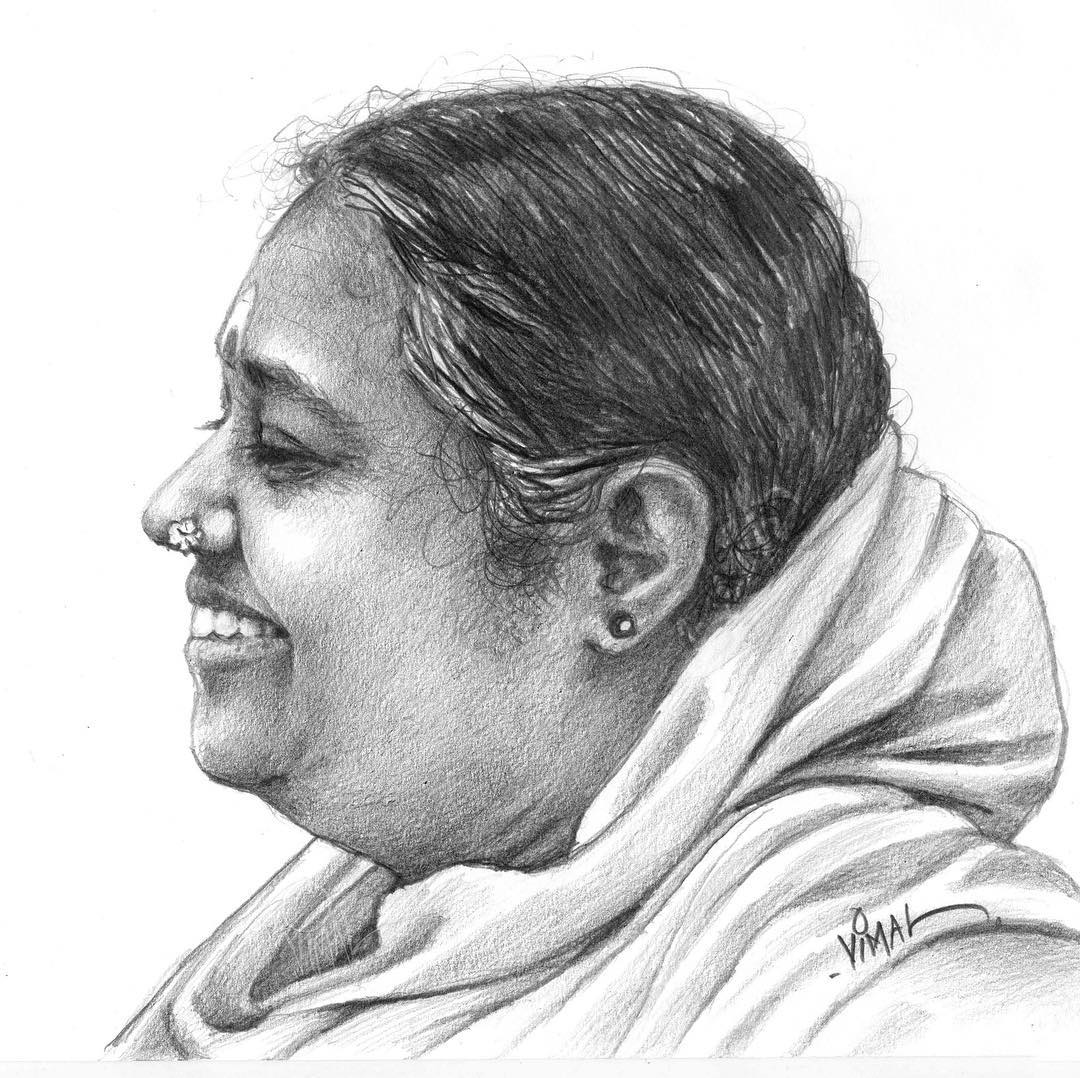
\includegraphics[width=0.25\paperwidth]{figs/amma.png}
    };
    \node[above left,inner sep= 0pt] at (current page.south east)
    {
        
\includegraphics[width=0.34\paperwidth]{figs/amritauniversity.eps}
    };
% Background image
    \node[above right,inner sep=0pt] at (current page.south west)
    {
        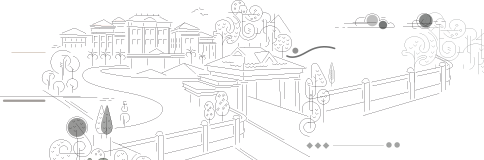
\includegraphics[width=0.44\paperwidth]{figs/amritapuricampus.png}
    };
    
% Title & Subtitle
\node
[
    above=1cm,
    align=center,
    fill= pantone!98!,
    rounded corners,
    inner xsep=10pt,
    inner ysep=10pt, 
    text = white,
    minimum width=0.25\textwidth,
    text width=0.85\textwidth,
] (title) at (current page.center)
{
\large \textsc{Presentation Title - Your Research}\\[5pt]
    %\small Subtitle of presentation
};   
% Author 
\node[ below=0.30cm] (author) at (title.south){\normalsize \textcolor{pantone}{NAME}};
\node[ below=0.9cm] (rollno) at (title.south){\scriptsize Roll No : AM.EN.P2WNA15151};
% \node[ below=1.3 cm] (mail) at (title.south){\scriptsize \ding{41} : \textit{dhaneshraj@am.amrita.edu}};
\node[ below=1.5 cm] (mail) at (title.south){\footnotesize Advisors : \textcolor{pantone}{Dr. Maneesha Vinodini Ramesh}\scriptsize{\textsuperscript{\ding{172}}}, \textcolor{pantone}{Dr. Sajal K Das}\scriptsize{\textsuperscript{\ding{173}}}};
% \node[ below=2.1 cm] (mail) at (title.south){\scriptsize Dr. Sajal K Das\ding{173}};
\node[ below= 2cm] (inst) at (title.south){\scriptsize{\textsuperscript{\ding{172}}}\scriptsize Center for Wireless Networks and Applications, Amrita Vishwa Vidyapeetham};
\node[ below= 2.4cm] (inst) at (title.south){\scriptsize{\textsuperscript{\ding{173}}}\scriptsize Missouri University of Science and Technology
};
\node[below=2.9cm] (date) at (title.south){\scriptsize \today};
% %%%%%%%%%%%%%%%%%%%%%%%%%%%%%%%%%%%%%%%%%%%%%%%%%%%%%%%%%%%%%%%%%%%%%%%%%%%%%%%%%
% ░E░░N░░D░ ░O░░F░ ░S░░I░░L░░D░░E░ ░SEVEN░░N░░E░
% %%%%%%%%%%%%%%%%%%%%%%%%%%%%%%%%%%%%%%%%%%%%%%%%%%%%%%%%%%%%%%%%%%%%%%%%%%%%%%%%%
% % Logo
% \node
% [
%     below right =0.25cm and 0.5cm
% ] at (current page.north west)
% {
%     \includegraphics[width=3.5cm]{pics/oceannetLogo.png}
% };

\end{tikzpicture}
\end{frame}
% %%%%%%%%%%%%%%%%%%%%%%%%%%%%%%%%%%%%%%%%%%%%%%%%%%%%%%%%%%%%%%%%%%%%%%%%%%%%%%%%%
% ░E░░N░░D░ ░O░░F░ ░S░░I░░L░░D░░E░ ░SEVEN░░N░░E░
% %%%%%%%%%%%%%%%%%%%%%%%%%%%%%%%%%%%%%%%%%%%%%%%%%%%%%%%%%%%%%%%%%%%%%%%%%%%%%%%%%
\begin{frame}
        \frametitle{\MakeUppercase{\textbf{\textsc{Outline}}}}
        \tableofcontents
        \addcontentsline{toc}{section}{First Section}
\end{frame}
% Outline frame
% %%%%%%%%%%%%%%%%%%%%%%%%%%%%%%%%%%%%%%%%%%%%%%%%%%%%%%%%%%%%%%%%%%%%%%%%%%%%%%%%%
% ░E░░N░░D░ ░O░░F░ ░S░░I░░L░░D░░E░ ░SEVEN░░N░░E░
% %%%%%%%%%%%%%%%%%%%%%%%%%%%%%%%%%%%%%%%%%%%%%%%%%%%%%%%%%%%%%%%%%%%%%%%%%%%%%%%%%
\section{Motivation} 
\begin{frame}{Motivation}
\centering
    
\includegraphics[scale=0.3]{figs/research.png}
\begin{exampleblock}{}
  { ``Hundreds of fishermen lose life every year in the sea due to non-availability of modern connectivity technologies, including satellite-based navigation system !''}
\end{exampleblock}
\end{frame}
%%%%%%%%%%%%%%%%%%%%%%%%%%%%%%%%%%%%%%%%%%%%%%%%%%%%%%%%%%%%%%%%%%%%%%%%%%%%%%%%%
% ░E░░N░░D░ ░O░░F░ ░S░░I░░L░░D░░E░ ░SEVEN░░N░░E░
%%%%%%%%%%%%%%%%%%%%%%%%%%%%%%%%%%%%%%%%%%%%%%%%%%%%%%%%%%%%%%%%%%%%%%%%%%%%%%%%%
\section{Introduction} 
\begin{frame}
\frametitle{Introduction}
\setbeamertemplate{itemize items}{\ding{97}}
\begin{itemize}
\justifying
\item Narrow Your Topic
\item Evaluate Your Topic
\item Vary your sources
\setbeamertemplate{itemize items}{\ding{47}}
\begin{itemize}
\item Refer to the notes section below  for guidelines on this topic
\pause
\item Refer to the notes section below  for guidelines on this topic
\end{itemize}
\end{itemize}
\end{frame}
%%%%%%%%%%%%%%%%%%%%%%%%%%%%%%%%%%%%%%%%%%%%%%%%%%%%%%%%%%%%%%%%%%%%%%%%%%%%%%%%%%░E░░N░░D░ ░O░░F░ ░S░░I░░L░░D░░E░ ░SEVEN░░N░░E░
%%%%%%%%%%%%%%%%%%%%%%%%%%%%%%%%%%%%%%%%%%%%%%%%%%%%%%%%%%%%%%%%%%%%%%%%%%%%%%%%%%
\section{Internet of Things} 
\begin{frame}
\frametitle{Challenges}
\begin{block}{Challenges in  IoT Networks}
\begin{itemize}
    \item Challenge 1
    \pause
    \item Challenge 2
    \pause
\end{itemize}
\end{block}
\transboxin
\end{frame}
% %%%%%%%%%%%%%%%%%%%%%%%%%%%%%%%%%%%%%%%%%%%%%%%%%%%%%%%%%%%%%%%%%%%%%%%%%%%%%%%%%
% ░E░░N░░D░ ░O░░F░ ░S░░I░░L░░D░░E░ ░SEVEN░░N░░E░
% %%%%%%%%%%%%%%%%%%%%%%%%%%%%%%%%%%%%%%%%%%%%%%%%%%%%%%%%%%%%%%%%%%%%%%%%%%%%%%%%%
\begin{frame}
\frametitle{Work in Brief}
\begin{block}{Research Objectives}
\begin{itemize}
    \item Objective 1
    \item Objective 2
\end{itemize}
\end{block}
\transboxin
\begin{alertblock}{Contributions}
\begin{enumerate}
    \item Literature Review on Current IoT, Fog and Cloud 
    \item Experimental Evaluation of 
\end{enumerate}
\end{alertblock}
\end{frame}
% %%%%%%%%%%%%%%%%%%%%%%%%%%%%%%%%%%%%%%%%%%%%%%%%%%%%%%%%%%%%%%%%%%%%%%%%%%%%%%%%%
% ░E░░N░░D░ ░O░░F░ ░S░░I░░L░░D░░E░ ░SEVEN░░N░░E░
% %%%%%%%%%%%%%%%%%%%%%%%%%%%%%%%%%%%%%%%%%%%%%%%%%%%%%%%%%%%%%%%%%%%%%%%%%%%%%%%%%
\begin{frame}
\frametitle{Literature Review}
\begin{block}{A Study on Marine Fog IoT Networks}
\begin{itemize}
    \item Marine Networks
        \begin{itemize}
        \item Research Gaps
            \begin{enumerate}
              \item Gap 1
              \item Gap 2
              \item Gap 3
            \end{enumerate}
        \item Investigation
            \begin{enumerate}
              \item Understanding the characteristics
              \item Enhancing QoS Delivery
              \item Inferring the QoS Tasks and minimizing delay \cite{Ref1}
            \end{enumerate}
        \item Proposed Research Outcome
            \begin{enumerate}
              \item Study on QoS and analysis of Challenged Networks \cite{Ref2}
              \item Architectural for Fog Assisted Marine IoT
              \item A method to improve the QoS
          \end{enumerate}
      \end{itemize}
\end{itemize}
\end{block}
\end{frame}
% %%%%%%%%%%%%%%%%%%%%%%%%%%%%%%%%%%%%%%%%%%%%%%%%%%%%%%%%%%%%%%%%%%%%%%%%%%%%%%%%%
% ░E░░N░░D░ ░O░░F░ ░S░░I░░L░░D░░E░ ░SEVEN░░N░░E░
% %%%%%%%%%%%%%%%%%%%%%%%%%%%%%%%%%%%%%%%%%%%%%%%%%%%%%%%%%%%%%%%%%%%%%%%%%%%%%%%%%
\begin{frame}
\resizebox{\columnwidth}{!}{%
\begin{tabular}{|llllll|}
\toprule
\thead{Study, Setting and \\ Sample Size} & \thead{Study Design} & \thead{Summary of Intervention} & \thead{Health System \\ Building Blocks \\ Included} & \thead{Summary of Findings} & \thead{Risk of Bias \\ Assessment} \\

\hline
\rowcolor{lightgray}
Column 1 Row 1 & Column 2 Row 1 & Column 3 Row 1 & Column 4 Row 1 & Column 5 Row 1 & Column 6 Row 1 \\
Column 1 Row 2 & Column 2 Row 2 & Column 3 Row 2 & Column 4 Row 2 & Column 5 Row 2 & Column 6 Row 2 \\
\rowcolor{lightgray}
Column 1 Row 3 & Column 2 Row 3 & Column 3 Row 3 & Column 4 Row 3 & Column 5 Row 3 & Column 6 Row 3 \\
Column 1 Row 4 & Column 2 Row 4 & Column 3 Row 4 & Column 4 Row 4 & Column 5 Row 4 & Column 6 Row 4 \\
\bottomrule
doc:10.137 & &  & & & \\
\end{tabular}
}

\end{frame}
% %%%%%%%%%%%%%%%%%%%%%%%%%%%%%%%%%%%%%%%%%%%%%%%%%%%%%%%%%%%%%%%%%%%%%%%%%%%%%%%%%
% ░E░░N░░D░ ░O░░F░ ░S░░I░░L░░D░░E░ ░SEVEN░░N░░E░
% %%%%%%%%%%%%%%%%%%%%%%%%%%%%%%%%%%%%%%%%%%%%%%%%%%%%%%%%%%%%%%%%%%%%%%%%%%%%%%%%%
\begin{frame}{Frame Title}
\begin{columns}[c] % t,b,h
\column{.55\textwidth}
\begin{block}{Block Title}
This is your Text
\end{block}
\pause %Use the \pause command to make items appear on a slid
\column{.35\textwidth}

\includegraphics[scale =0.2]{figs/research1.png}
\end{columns}
\end{frame}
\begin{frame}{Plan for completion and thesis submission}
\footnotesize
\setlength\tabcolsep{4pt} % default: 6pt
\begin{tabularx}{\textwidth}{@{}>{\RaggedRight}X*{5}{c}@{}}
\toprule
Tasks & \multicolumn{2}{c}{2016--17} & \multicolumn{2}{c}{2017--18} & 2018--19\\
\cmidrule(l){2-6}
& {\tiny Sem.\ 1} & {\tiny Sem.\ 2} & {\tiny Sem.\ 1} & {\tiny Sem.\ 2} & {\tiny Sep--Dec 18} \\
\midrule
Reading and understanding of various advanced concepts on groups and graphs 
& $\times$ & $\times$  \\
\addlinespace
Write a literature review 
& $\times$ \\
\addlinespace
Obtain examples (by hand or using a computational algebra system)    
& & $\times$ \\
\addlinespace
Form conjectures and prove or disprove the conjectures 
& & $\times$ \\
\addlinespace
Work on research problems 
& & $\times$ &$\times$ & $\times$ & $\times$ \\
\addlinespace
Submit a paper to an ISI-indexed journal for publication
& & & $\times$ \\ 
\addlinespace
Write up thesis for submission 
& & & &$\times$ \\
\addlinespace
Complete writing up of thesis and submit thesis by December 2018 
& & & & & $\times$ \\
\bottomrule
\end{tabularx}
\end{frame}
% %%%%%%%%%%%%%%%%%%%%%%%%%%%%%%%%%%%%%%%%%%%%%%%%%%%%%%%%%%%%%%%%%%%%%%%%%%%%%%%%%
% ░E░░N░░D░ ░O░░F░ ░S░░I░░L░░D░░E░ ░SEVEN░░N░░E░
% %%%%%%%%%%%%%%%%%%%%%%%%%%%%%%%%%%%%%%%%%%%%%%%%%%%%%%%%%%%%%%%%%%%%%%%%%%%%%%%%%
\begin{frame}[allowframebreaks]
\def\newblock{}
\frametitle{References}
  \bibliographystyle{plain}
  \bibliography{references.bib}
\end{frame}
% %%%%%%%%%%%%%%%%%%%%%%%%%%%%%%%%%%%%%%%%%%%%%%%%%%%%%%%%%%%%%%%%%%%%%%%%%%%%%%%%%
% ░E░░N░░D░ ░O░░F░ ░S░░I░░L░░D░░E░ ░SEVEN░░N░░E░
% %%%%%%%%%%%%%%%%%%%%%%%%%%%%%%%%%%%%%%%%%%%%%%%%%%%%%%%%%%%%%%%%%%%%%%%%%%%%%%%%%
\begin{frame}
\Huge{\centerline{THANK YOU}}
\end{frame}
% %%%%%%%%%%%%%%%%%%%%%%%%%%%%%%%%%%%%%%%%%%%%%%%%%%%%%%%%%%%%%%%%%%%%%%%%%%%%%%%%%
% ░E░░N░░D░ ░O░░F░ ░S░░I░░L░░D░░E░ ░SEVEN░░N░░E░
% %%%%%%%%%%%%%%%%%%%%%%%%%%%%%%%%%%%%%%%%%%%%%%%%%%%%%%%%%%%%%%%%%%%%%%%%%%%%%%%%%
%----------------------------------------------------------------------------------------
\end{document}